\documentclass[hyperref={pdfpagelabel=false},usepdftitle=false,xcolor=dvipsnames]{beamer}

\usepackage[T3]{fontenc}
\usepackage[utf8]{inputenc}
\usepackage[russian]{babel}

\usepackage{mhchem}
\usepackage{amssymb, amsmath}

\usepackage{tikz}
\usetikzlibrary{shapes.geometric, arrows, positioning, decorations.markings}
\usetikzlibrary{fit}
\usepackage{microtype}
\usepackage{framed}
\usetikzlibrary{decorations.pathmorphing,calc,backgrounds}

\usepackage{animate}

\usepackage{fixltx2e}
\usepackage{hyperref}

%\usetheme{Berkeley}
%\usetheme{Madrid} -- неплохо
%\usetheme{CambridgeUS}
%\usetheme{Singapore}
\usetheme{Warsaw}

\pdfmapfile{+sansmathaccent.map}

\title{Исследование бифуркаций в трехатомных гидридах методом классических траекторий}

\author{\small 
Финенко Артем \\[1ex] 
Научный руководитель: Петров С.В.}

\institute[MSU] % (optional, but mostly needed)
{
  МГУ им. М.В.Ломоносова \\
  Химический факультет
}

\date{23/12/2016}

\pgfdeclareimage[height=0.5cm]{university-logo}{../pictures/logo.jpg}
\logo{\pgfuseimage{university-logo}}

\newcommand\Fontvi{\fontsize{6}{7.2}\selectfont}

\beamertemplatenavigationsymbolsempty

\setbeamerfont{page number in head/foot}{size=\large}
\setbeamertemplate{footline}[frame number]
\setbeamertemplate{frametitle}[default][center]

% change font
\usefonttheme[onlymath]{serif}

% custom block environment
\newenvironment<>{varblock}[2][.9\textwidth]{%
  \setlength{\textwidth}{#1}
  \begin{actionenv}#3%
    \def\insertblocktitle{#2}%
    \par%
    \usebeamertemplate{block begin}}
  {\par%
    \usebeamertemplate{block end}%
  \end{actionenv}}

\tikzstyle{lagrange} = [rectangle, rounded corners, minimum width = 3cm, minimum height = 1cm, text centered, text width = 5cm, draw = black, fill=DarkOrchid!40]

\tikzstyle{equations} = [rectangle, rounded corners, text centered, draw = black, fill=green!30]

\tikzstyle{hamilton} = [rectangle, rounded corners, minimum width = 3cm, minimum height = 1cm, text centered, text width = 5 cm, draw = black, fill = Goldenrod!50]

\tikzstyle{result} = [rectangle, rounded corners, text centered, draw = black, fill = blue!30]

\tikzstyle{arrow} = [thick, ->, >=stealth]

\tikzstyle{vecArrow} = [thick, decoration={markings,mark=at position
   1 with {\arrow[semithick]{open triangle 60}}},
   double distance=1.4pt, shorten >= 5.5pt,
   preaction = {decorate},
   postaction = {draw,line width=1.4pt, white,shorten >= 4.5pt}]

\usepackage{caption}
\usepackage{subcaption}

\newcommand{\mL}{\mathcal{L}}
\newcommand{\mH}{\mathcal{H}}
\newcommand{\mf}{\mathbf}
\newcommand{\lb}{\left(}
\newcommand{\rb}{\right)}

\usepackage{dsfont}
\usepackage{bbm}
\newcommand{\bbI}{\mathds{I}}
\newcommand{\bba}{\mathbbm{a}}
\newcommand{\bbA}{\mathds{A}}
\newcommand{\bbB}{\mathds{B}}
\newcommand{\bbG}{\mathds{G}}

\usepackage{graphicx}

% custom block environment
\newenvironment<>{varblock}[2][.9\textwidth]{%
  \setlength{\textwidth}{#1}
  \begin{actionenv}#3%
    \def\insertblocktitle{#2}%
    \par%
    \usebeamertemplate{block begin}}
  {\par%
    \usebeamertemplate{block end}%
  \end{actionenv}}

\begin{document}

\begin{frame}
{
\vspace*{-0.75cm}
\large 
\begin{center}
Кафедра физической химии \\
Лаборатория строения и квантовой механики молекул
\vspace*{-0.75cm}
\end{center}}
 \titlepage
\end{frame}

\begin{frame}{\normalsize Классический колебательно-вращательный гамильтониан \rom{1}}
\begin{tikzpicture}[framed, font=\sffamily\small]

\node (lag1) [lagrange, text width = 2.5cm] {\scalebox{.8}{$T_\mL = \displaystyle\frac{1}{2}\sum_{i=1}^{n} m_i \dot{\mf{r}}_i^2$}};

\node (lag2) [lagrange, text width = 7cm, below = 1 cm of lag1] {\scalebox{.8}{$T_\mL = \displaystyle\frac{1}{2} \sum_{i=1}^{n} m_i \dot{\mf{R}}_i^2 + \mf{\Omega}^{\top} \sum_{i=1}^{n} m_i \left[ \mf{R}_i \times \dot{\mf{R}}_i \right] + \frac{1}{2} \mf{\Omega}^\top \bbI \, \mf{\Omega}$}};

\node (lag3) [lagrange, text width = 7 cm, below = 1.5 cm of lag2] {\scalebox{.8}{$
\begin{aligned}
	& \quad \quad T_\mL = \displaystyle\frac{1}{2} \dot{\mf{q}}^\top \bba \, \dot{\mf{q}} + \mf{\Omega}^\top \bbA \, \mf{\dot{q}} + \frac{1}{2} \mf{\Omega}^\top \bbI \, \mf{\Omega} \\
	\bba_{jk} &= \sum_{i=1}^{n} m_i \frac{\partial \mf{R}_i}{\partial q_j} \frac{\partial \mf{R}_i}{\partial q_k}, \quad \bbA_{jk} = \sum_{i=1}^{n} m_i \hspace*{-0.1cm} \left[ \mf{R}_i \times \frac{\partial \mf{R}_i}{\partial q_k} \right]_j 
\end{aligned}$
}};

\node (eq1) [equations, minimum width = 2cm, text width = 2cm, below right = 0.1 cm and 2 cm of lag1] {$\mf{R}_i = \mathbb{S} \mf{r}_i$};

\node (eq2) [equations, minimum width = 3cm, text width = 3cm, below right = 0.1 cm and -0.5 cm of lag2] {$
\begin{aligned}
	\mf{R}_i &= \mf{R}_i \lb \mf{q} \rb \\
	\mf{q} &= \lb q_1, \dots, q_n \rb
\end{aligned}$};

\draw [vecArrow] (lag1) -- node (text1) [anchor = east, text width = 5cm] {\vspace*{-0.5cm} \begin{center}Переход в подвижную систему отсчета \end{center}} (lag2);

\draw [vecArrow] (lag2) -- node (text2) [anchor = east, text width = 5cm] {\vspace*{-0.5cm} \begin{center}Переход к обобщенным координатам\end{center}} (lag3);

\draw [arrow] (lag1) -| (eq1);
\draw [arrow] (eq1) |- ([yshift=4pt]lag2);
\draw [arrow] ([yshift=-4pt]lag2) -| (eq2);
\draw [arrow] (eq2) |- ([yshift=4pt]lag3);

\begin{scope}[on background layer]
  \node [fill = BurntOrange!20,fit= (lag1) (lag2) (lag3) (text1) (text2) (eq1) (eq2)] {};
\end{scope}
\end{tikzpicture}
\end{frame}

\begin{frame}{\normalsize Классический колебательно-вращательный гамильтониан \rom{2}}
\begin{tikzpicture}[framed, font=\sffamily\small]

\node (lag1) [lagrange, text width = 6cm] {\scalebox{.8}{$
T_\mL = \displaystyle\frac{1}{2}
\begin{bmatrix}
	\mf{\Omega}^\top & \hspace*{-0.3cm} \dot{\mf{q}}^\top
\end{bmatrix}
\bbB
\begin{bmatrix}
	\mf{\Omega} \\ \dot{\mf{q}}
\end{bmatrix},
\quad 
\bbB =
\begin{bmatrix}
	\bbI & \hspace*{-0.2cm} \bbA \\
	\hspace*{0.15cm} \bbA^\top & \hspace*{-0.25cm} \bba
\end{bmatrix}
$}};

\node (eq1) [equations, text width = 5cm, below right = 0.3cm and -2cm of lag1] {\scalebox{.8}{$
\begin{aligned}
	\mf{J} &= \displaystyle\frac{\partial T_\mL}{\partial \mf{\Omega}} = \bbI \, \mf{\Omega} + \bbA \, \dot{\mf{q}} \\
	\mf{p} &= \frac{\partial T_\mL}{\partial \dot{\mf{q}}} = \bbA^\top \Omega + \bba \, \dot{\mf{q}}
\end{aligned}
\quad
\begin{bmatrix}
	\mf{J} \\
	\mf{p}
\end{bmatrix}
= \bbB
\begin{bmatrix}
	\mf{\Omega} \\
	\dot{\mf{q}}
\end{bmatrix}
$}};

\node (ham1) [hamilton, text width = 7.5cm, below = 2.2cm of lag1] {\scalebox{.8}{$
\begin{aligned}
&T_\mH = 
\begin{bmatrix}
	\mf{\Omega}^\top & \hspace*{-.25cm} \dot{\mf{q}}^\top
\end{bmatrix}
\begin{bmatrix}
	\mf{J} \\
	\mf{p}
\end{bmatrix}
- T_\mL = \displaystyle\frac{1}{2}
\begin{bmatrix}
	\mf{J}^\top & \hspace*{-.25cm} \mf{p}^\top
\end{bmatrix}
\bbG
\begin{bmatrix}
	\mf{J} \\
	\mf{p}
\end{bmatrix},
\quad
\bbG = \bbB^{-1} \\
& \quad \quad T_\mH = \frac{1}{2} \mf{J}^\top \bbG_{11} \, \mf{J} + \mf{J}^\top \bbG_{12} \, \mf{p} + \frac{1}{2} \mf{p}^\top \bbG_{22} \, \mf{p} \\
& \hspace*{2.5cm} \bbG_{11} = \lb \bbI - \bbA \bba^{-1} \bbA^\top \rb^{-1} \\
& \hspace*{2.5cm} \bbG_{12} = - \bbI^{-1} \bbA \, \bbG_{22} = - \bbG_{11} \bbA \bba^{-1} \\
& \hspace*{2.5cm} \bbG_{21} = - \bba^{-1} \bbA^\top \bbG_{11} = \bbG_{22} \, \bbA^\top \bbI^{-1} \\
& \hspace*{2.5cm} \bbG_{22} = \lb \bba - \bbA^\top \bbI^{-1} \bbA \rb^{-1}
\end{aligned}
$}};
	
\draw [vecArrow] (lag1) -- node (text1) [anchor = east, text width = 5cm] {\vspace*{-0.5cm} \begin{center} Применение \\ теоремы Донкина \end{center}} (ham1);

	\draw [arrow] (lag1) -| ([xshift=30pt]eq1);
	\draw [arrow] ([xshift=60pt]eq1) |- (ham1); 

\begin{scope}[on background layer]
	\node [fill = BurntOrange!20, fit = (lag1) (eq1) (ham1) (text1)] {};	
\end{scope}
\end{tikzpicture}
\end{frame}

\begin{frame}{\normalsize Точный классический колебательно-вращательный гамильтониан системы $Ar-CO_2$ \rom{1}}
\begin{figure}
\begin{tikzpicture}
	[oxygen/.style={ball color = red, circle, text = white}, 
	carbon/.style={ball color = black!30, circle, text = white},
	argon/.style={ball color = blue, circle, text = white}]
	\node (z1) at (4.5, 3) {OZ};
	\node (z2) at (-1.5, -1) {}
		edge [->, thick] (z1);

	\node (x1) at (-1, 3.5) {OX};
	\node (x2) at (3.5, -1) {}
		edge [->, thick] (x1); 

	\node (carbon) [carbon] {C};
	\node (oxygen1) [oxygen, below right of = carbon] {O}
		edge [double, thick] (carbon);
	\node (oxygen2) [oxygen, above left of = carbon] {O}
		edge [double, thick] (carbon);
	\node[argon] (argon) at (3, 2) {Ar};
\begin{scope}[on background layer]
	\node [fill=BurntOrange!20,fit=(z1) (z2) (x1) (x2) (carbon) (oxygen1) (oxygen2)] {};
\end{scope}
\end{tikzpicture}
\caption{\centering Молекулярная система координат для системы $Ar-CO_2$}
\end{figure}
\end{frame} 

\begin{frame}{\normalsize Точный классический колебательно-вращательный гамильтониан системы $Ar-CO_2$ \rom{2}}

	Обозначим массы атомов: кислорода -- $m_1$, аргона -- $m_2$, углерода -- $m_3$, обозначим через $l$ расстояние $O-O$ в молекуле $CO_2$, расстояние от атома $C$ до атома $Ar$ -- через $R$, угол между вектором $C-Ar$ и $CO_2$ -- через $\theta$. Пара переменных $R, \theta$ образуют систему внутренних координат.  
	
\begin{block}{}
\begin{gather}
	\scalebox{.8}{$\hspace*{-2cm} \mH = \displaystyle\frac{1}{2 \mu_2} p_R^2 + \lb \frac{1}{2 \mu_2 R^2} + \frac{1}{2 \mu_1 l^2} \rb p_\theta^2 - \frac{1}{\mu_2 R^2} p_\theta J_y + \frac{1}{2 \mu_2 R^2} J_y^2 + \frac{1}{2 \mu_2 R^2} J_x^2 + $} \notag \\
	\scalebox{.8}{$\hspace*{5cm} \displaystyle + \frac{1}{2 \sin^2 \theta} \lb \frac{\cos^2 \theta}{\mu_2 R^2} + \frac{1}{\mu_1 l^2} \rb J_z^2 + \frac{\ctg \theta}{\mu_2 R^2} J_x J_z + U(R, \theta) $} \notag \\
	\scalebox{.8}{$ \displaystyle \mu_1 = \frac{m_1}{2}, \quad \mu_2 = \frac{m_2 \lb 2 m_1 + m_3 \rb}{2 m_1 + m_2 + m_3}$} \notag
\end{gather}
\end{block}
\end{frame}

\begin{frame}{\normalsize Поверхность потенциальной энергии межмолекулярного взаимодействия}
\vspace*{-0.30cm}
\begin{figure}
	\hspace*{-1cm}
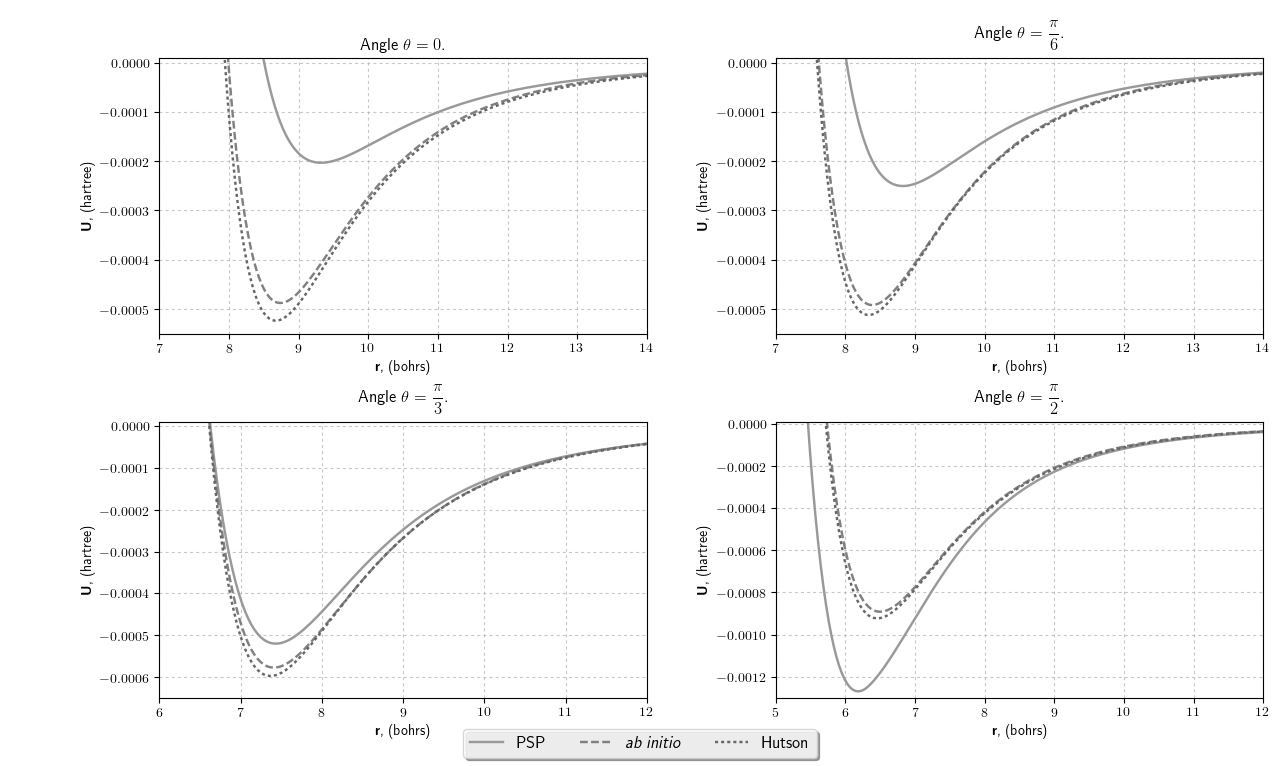
\includegraphics[width = \linewidth]{../pictures/potential_well.png}
\vspace*{-0.1cm}
\caption{\centering \scriptsize Сечения поверхностей потенциальной энергии при разных углах $\theta$ в области потенциальной ямы}
\end{figure}
\end{frame}

\begin{frame}{\normalsize Второй вириальный коэффициент и первые квантовые поправки для системы $Ar-CO_2$ \rom{1}}
\begin{block}{\scriptsize ВВК для молекулярных систем с внутренними степенями свободы}
\begin{gather}
	\scalebox{0.8}{$B_2 = \displaystyle \frac{N_A}{2 V} \frac{\iint_{\lb \tau \rb} f_{12} \, d \tau_1 \, d \tau_2}{\int d \Omega_1 \int d \Omega_2}, \quad d \tau_i = d \mf{r}_i \, d \Omega_i  $} \notag
\end{gather}
\end{block}

\begin{block}{\scriptsize ВВК для системы $Ar-CO_2$} 
\begin{gather}
	\scalebox{0.8}{$\displaystyle B_2 = \frac{N_A}{2 V} \frac{\iint_{\lb \tau \rb} \lb 1 - \exp \lb - \beta U \lb \mf{r}_1, \mf{r}_2, \theta \rb \rb \rb \,  d \mf{r}_1 \, d \mf{r}_2 \, \sin \theta d \theta}{ \int d \Omega_1} = \hspace*{5cm} $} \notag\\ 
	\scalebox{0.8}{$ \hspace{5cm} = \displaystyle \pi N_A \int\limits_{0}^{\infty} \int\limits_{0}^{\pi} \lb 1 - \exp \lb - \beta U \lb R, \theta \rb \rb \rb R^2 d R \, \sin \theta \, d \theta$} \notag
\end{gather}
\end{block}
\end{frame}


\begin{frame}{\normalsize Расчет температурной зависимости второго вириального коэффициента для системы $Ar-CO_2$ \rom{2}}
\vspace*{-0.35cm}
\begin{figure}
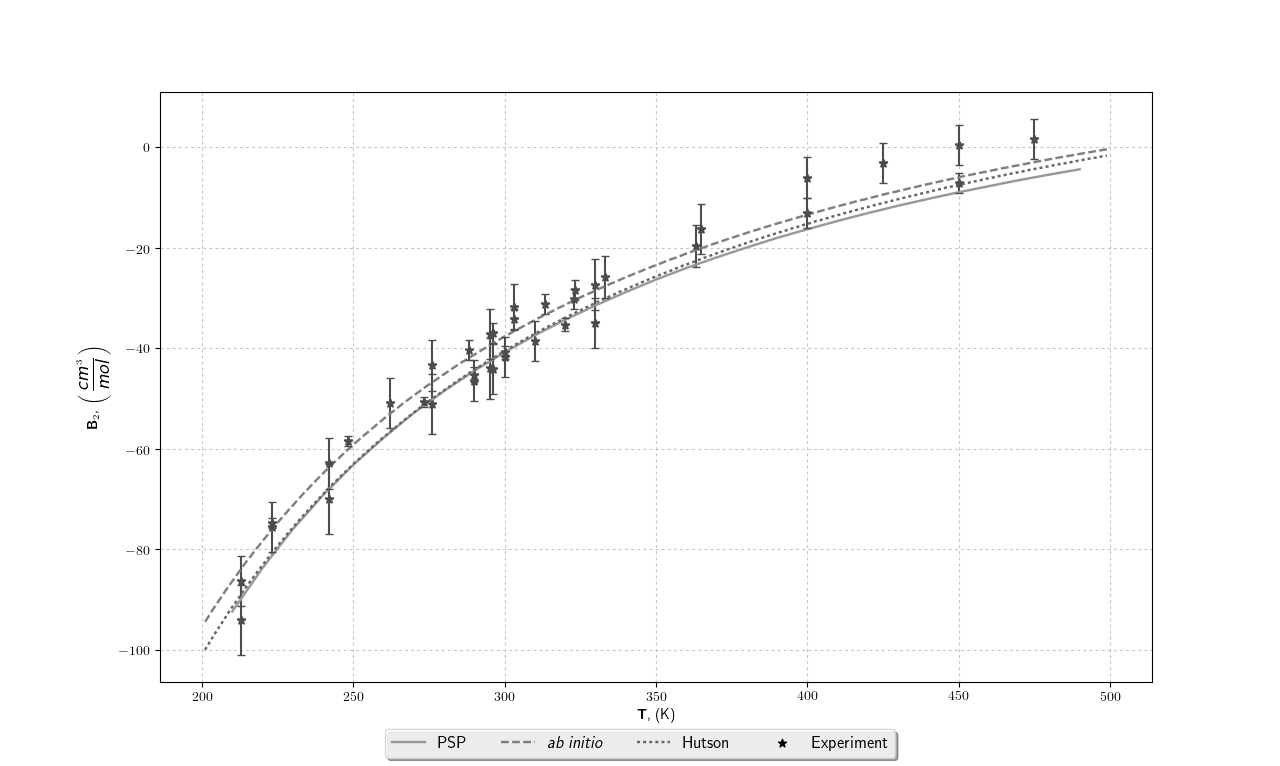
\includegraphics[width=\linewidth]{../pictures/virexpmod.png}
\vspace*{-0.35cm}
\caption{\centering \scriptsize Температурные зависимости вириальных коэффициентов для разных ППЭ}
\end{figure}
\end{frame}

\begin{frame}{\normalsize Расчет температурной зависимости второго вириального коэффициента для системы $Ar-CO_2$ \rom{3}}
\vspace*{-0.35cm}
\begin{figure}
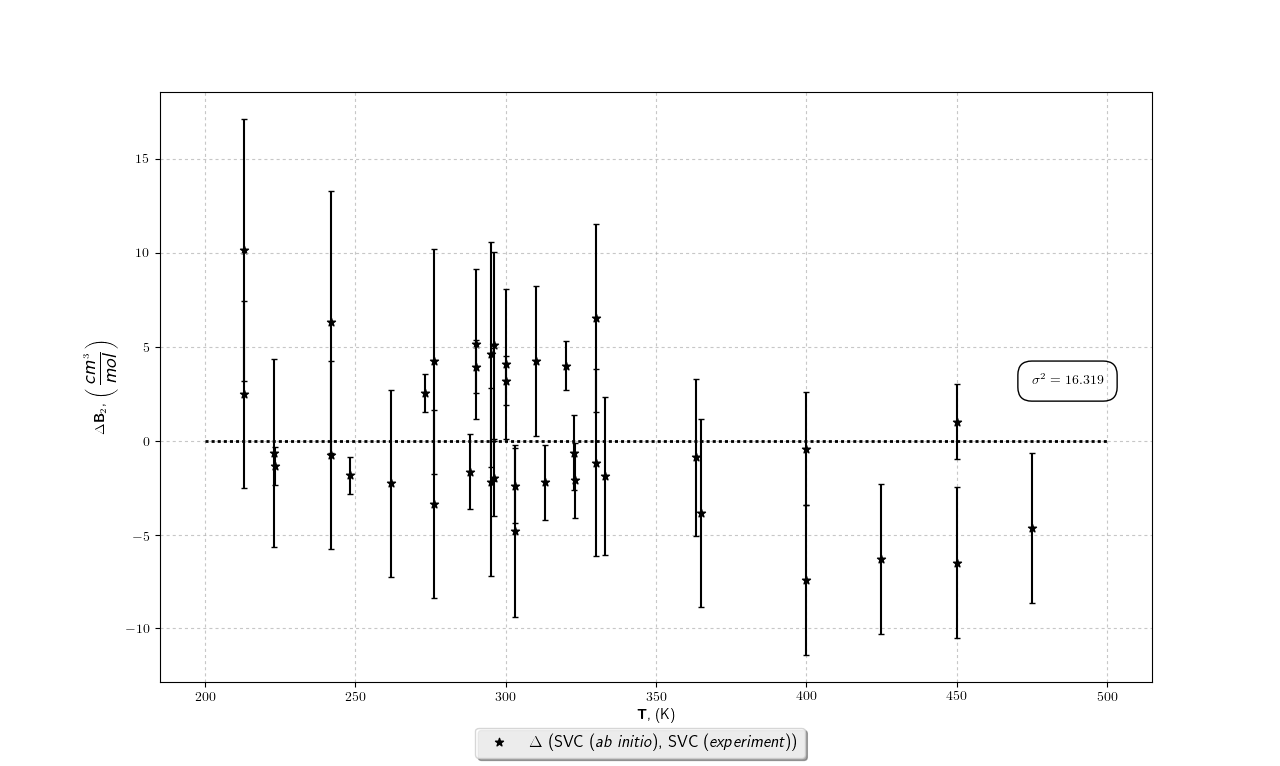
\includegraphics[width=\linewidth]{../pictures/virdeltaab.png}
\vspace*{-0.45cm}
\caption{\centering \scalebox{0.62}{Разница между экспериментальными значениями ВВК и значениями, рассчитанными для \textit{ab initio} потенциала}}
\end{figure}
\end{frame}

\begin{frame}{\normalsize Расчет температурной зависимости второго вириального коэффициента для системы $Ar-CO_2$ \rom{4}}
\begin{block}{\scriptsize Разложение Вигнера-Кирквуда}
\begin{gather}
\scalebox{0.8}{$ \displaystyle B = B_{\text{класс.}} + \frac{\hbar^2}{m} B_{t1} + \lb \frac{\hbar^2}{m} \rb^2 B_{t2} + \dots + \frac{\hbar^2}{I} B_{r1} + \lb \frac{\hbar^2}{I} \rb^2 B_{r2} + \dots $} \notag
\end{gather}
\end{block}
\begin{block}{\scriptsize Поправки в разложении Вигнера-Кирквуда для cистемы $Ar-CO_2$}
\begin{gather}
\scalebox{0.8}{$ \displaystyle B_{t1} = \frac{\pi N_A}{12 \lb k T \rb^3} \int\limits_{0}^{\infty} \int\limits_{0}^{\pi} \exp \lb - \frac{U}{k T} \rb \lb \frac{\partial U}{\partial R} \rb^2 R^2 \, d R \sin \theta \, d \theta $} \notag \\
\scalebox{0.8}{$ \displaystyle B_{r1} = \frac{\pi N_A}{24 \lb k T \rb^3} \int\limits_{0}^{\infty} \int\limits_{0}^{\pi} \exp \lb - \frac{U}{k T} \rb \lb \frac{\partial U}{\partial \theta} \rb^2 R^2 d R \sin \theta \, d \theta $} \notag
\end{gather}
\end{block}
\end{frame}

\begin{frame}{\normalsize Расчет температурной зависимости второго вириального коэффициента для системы $Ar-CO_2$ \rom{5}}
\vspace*{-0.35cm}
\begin{figure}
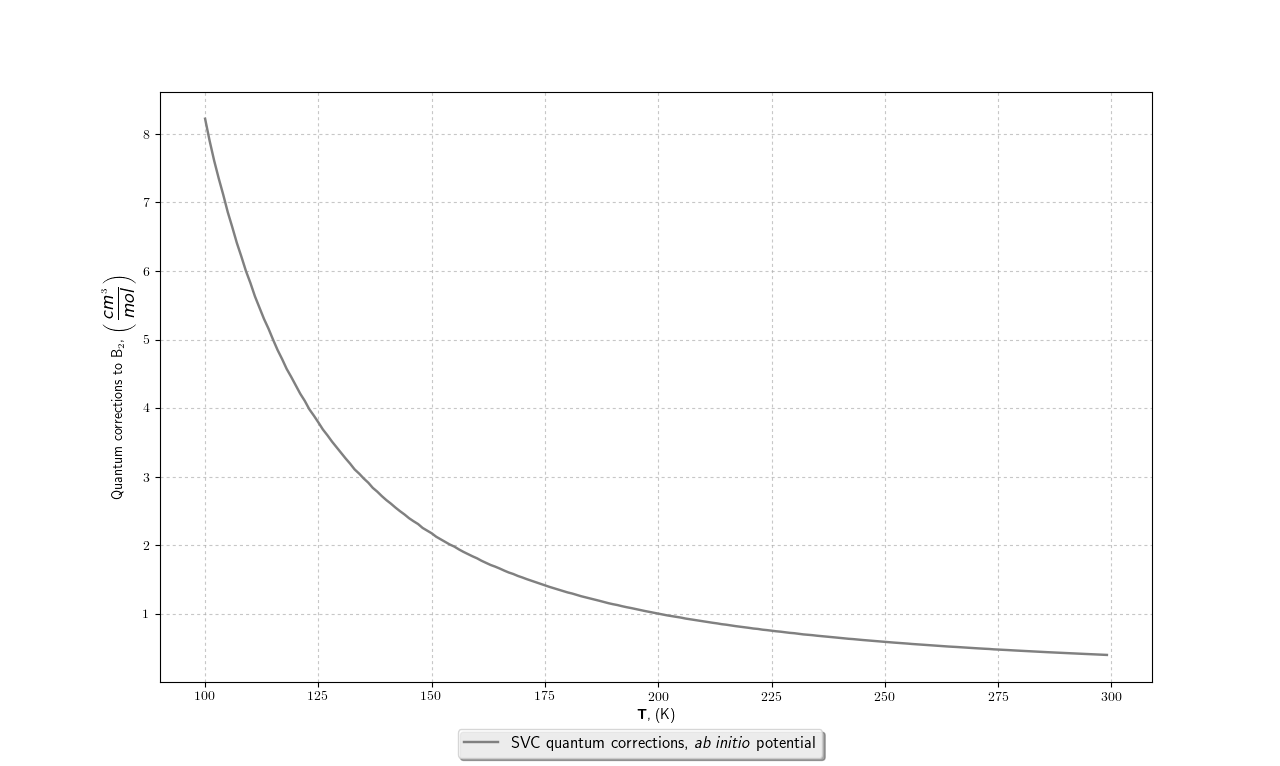
\includegraphics[width=\linewidth]{../pictures/vircorr2.png}
\vspace*{-0.42cm}
\caption{\centering \scalebox{0.8}{Вклад квантовых поправок в температурную зависимость ВВК для \textit{ab initio} потенциала}}
\end{figure}
\end{frame}

\begin{frame}{\normalsize Расчет температурной зависимости второго вириального коэффициента для системы $Ar-CO_2$ \rom{6}}
\vspace*{-0.35cm}
\begin{figure}
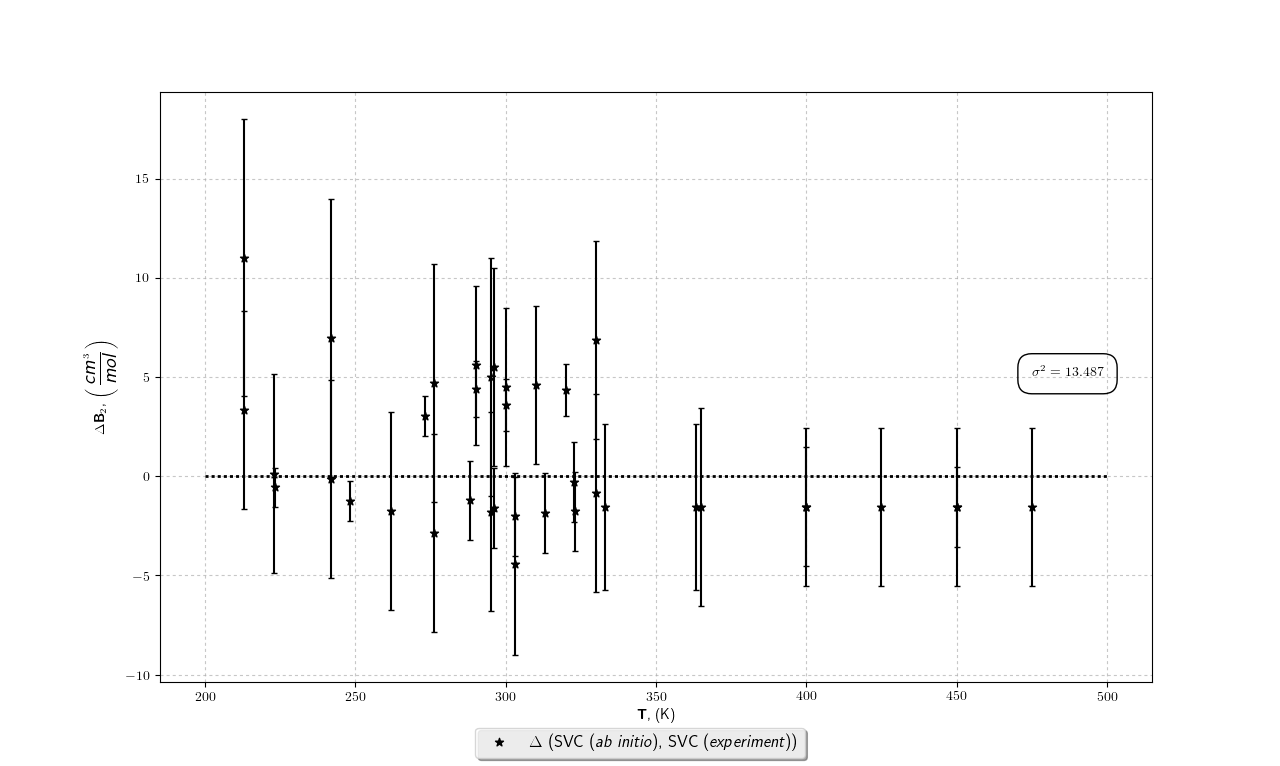
\includegraphics[width=\linewidth]{../pictures/virdeltaabcorr.png}
\vspace*{-0.40cm}
\caption{\centering \scalebox{0.63}{Разница между экспериментальными значениями ВВК и значениями, рассчитанными для \textit{ab initio} потенциала}}
\end{figure}
\end{frame}

\begin{frame}{\normalsize Константа равновесия слабосвязанного комплекса $Ar-CO_2$ \rom{1}}
	\begin{block}{\scriptsize Газовая константа равновесия $K_p$}
		\begin{gather}
			\scalebox{0.8}{$\displaystyle K_p = \frac{N_A}{p^{\barcirc}} \frac{Q_{bound}^{pair}}{Q_{Ar} Q_{CO_2}} $} \notag
		\end{gather}
	\end{block}
	\begin{block}{\scriptsize Сумма по состояниям связанного димера}
		\begin{gather}
			\scalebox{0.8}{$\displaystyle Q_{bound}^{pair} = \frac{1}{h^8} \int_{H - P_{cm}^2 / 2 M} \exp \lb -\frac{H}{kT} \rb d x_{cm} \, dy_{cm} \, d z_{cm} \, d P_x \, d P_y \, d P_z d q_i d p_i =$} \notag \\
			\scalebox{0.8}{$\displaystyle = \lb Q_{bound}^{pair} \rb_{tr} \frac{4 \pi^2}{h^5} \int_{\mH < 0} \exp \lb - \frac{\mH}{kT} \rb d R \, d \theta \, d p_R \, d p_\theta \, d J_x \, d J_y \, d J_z$} \notag
		\end{gather}
	\end{block}
	\begin{block}{\scriptsize Гамильтониан как положительно определенная квадратичная форма}
		\begin{gather}
			\scalebox{0.8}{$\displaystyle \mH = \frac{p_R^2}{2 \mu_2} + \frac{p_\theta^2}{2 \mu_1 l^2} + \frac{1}{2 \mu_2 R^2} \lb p_\theta - J_y \rb^2 + \frac{1}{2 \mu_2 R^2} \lb J_x + J_z \ctg \theta \rb^2 + \frac{J_z^2}{2 \mu_1 l^2 \sin^2 \theta} + U \lb R, \theta \rb$} \notag
		\end{gather}
	\end{block}
\end{frame}

\begin{frame}{\normalsize Константа равновесия слабосвязанного комплекса $Ar-CO_2$ \rom{2}}
	\hspace*{-0.25cm}
\begin{tikzpicture}[framed, font=\sffamily\small]
	\node (int1) [hamilton, text width = 7cm] {\scalebox{0.8}{$\displaystyle \frac{1}{h^5} \int_{\mH < 0} \exp \lb - \frac{\mH}{kT} \rb d R \, d p_R \, d \theta \, d p_\theta \, d J_x \, d J_y \, d J_z$}};

	\node (int2) [hamilton, text width = 7cm, below = 0.2cm of int1] {\scalebox{0.8}{$\displaystyle \frac{1}{h^5} \iint d R d \theta \int \exp \lb - \frac{\mH}{k T} \rb d p_R \, d p_\theta \, d J_x \, d J_y \, d J_z$}};

	\node (eq1) [equations, text width = 11.1cm, below right = 0.2cm and -9.25cm of int2] {\scalebox{0.8}{$\displaystyle x_1^2 = \frac{p_R^2}{2 \mu_2 k T}, \ x_2^2 = \frac{p_\theta^2}{2 \mu_1 l^2 k T}, \ x_3^2 = \frac{\lb p_\theta - J_y \rb^2}{2 \mu_2 R^2 k T}, \ x_4^2 = \frac{\lb J_x + J_z \ctg \theta \rb^2}{2 \mu_2 R^2 k T}, \ x_5^2 = \frac{J_z^2}{2 \mu_1 l^2 \sin^2 \theta k T} $}};

	\node (int3) [hamilton, text width = 11cm, below = 0.2cm of eq1] {\scalebox{0.8}{$\displaystyle \iint \left[ \textit{Jac} \, \right] \cdot \exp \lb - \frac{U}{k T} \rb d R d \theta \times \idotsint_{x_1^2 + \cdots x_5^2 \leqslant - U / kT} \exp \lb - x_1^2 - \dots - x_5^2 \rb d x_1 \, \dots d x_5$}}; 	

	\node (eq2) [equations, below = 0.2cm of int3] {\scalebox{0.8}{$\displaystyle \idotsint_{x_1^2 + \cdots + x_n^2 \leqslant R} \exp \lb -x_1^2 - \dots -x_n^2 \rb  = \pi^{n / 2} \frac{\gamma \lb \frac{n}{2}, R^2 \rb}{\Gamma \lb \frac{n}{2} \rb}, \quad \gamma (a, b) = \int\limits_{0}^{b} \omega^{a-1} \exp \lb - \omega \rb d \omega $}};

	\node (int4) [hamilton, text width = 9cm, below = 0.2cm of eq2] {\scalebox{0.8}{$\displaystyle \lb \frac{2 \pi \mu_2 k T}{h^2} \rb^{\frac{3}{2}} \frac{2 \mu_1 l^2 \pi k T}{h^2} \iint_{U < 0} \exp \lb -\frac{U}{k T} \rb \frac{\gamma \lb \frac{5}{2}, - \frac{U}{kT} \rb}{\Gamma \lb \frac{5}{2} \rb} R^2 \sin \theta \, d R \, d \theta$}};	

	\draw [arrow] (int1.west) to [out=180, in=180, anchor=east] node (text1) {\scalebox{0.7}{Т. Фубини}} ([yshift=5pt]int2.west);
	\draw [arrow] (int2.west) -| ([xshift=-300pt]eq1);
	\draw [arrow] ([xshift=-125pt]eq1.south) -- ([xshift=-125pt]int3.north);
	\draw [arrow] ([xshift=-125pt]int3.south) -- ([xshift=-125pt]eq2.north);
	\draw [arrow] ([xshift=-125pt]eq2.south) -- ([xshift=-125pt]int4.north);

\begin{scope}[on background layer]
	\node [fill=BurntOrange!20,fit=(int1) (int2) (int3) (int4) (eq1) (eq2)] {};
\end{scope}
\end{tikzpicture}
\end{frame}

\begin{frame}{\normalsize Константа равновесия слабосвязанного комплекса $Ar-CO_2$ \rom{3}}
	\begin{block}{Модифицированное выражение для константы равновесия}
		\begin{gather}
			\scalebox{0.8}{$\displaystyle K_p = \frac{2 \pi N_A}{RT} \iint_{U < 0} \exp \lb - \frac{U}{kT} \rb \frac{\gamma \lb \frac{5}{2}, - \frac{U}{kT} \rb}{\Gamma \lb \frac{5}{2} \rb} R^2 d R \, \sin \theta \, d \theta$} \notag
		\end{gather}
	\end{block}
	\begin{block}{Общее выражение для константы равновесия}
		\begin{gather}
			\scalebox{0.8}{$\displaystyle K_p = \frac{4 \pi^2 N_A}{R T} \frac{\lb Q_{bound}^{pair} \rb_{tr}}{Q_{Ar} Q_{CO_2}} \int_{\mH < 0} \exp \lb - \frac{\mH}{kT} \rb d R \, d \theta \, d p_R \, d p_\theta \, d J_x \, d J_y \, d J_z$} \notag
		\end{gather}
	\end{block}
\end{frame}

\begin{frame}{\normalsize Константа равновесия слабосвязанного комплекса $Ar-CO_2$ \rom{4}}
\vspace*{-0.35cm}
\begin{figure}
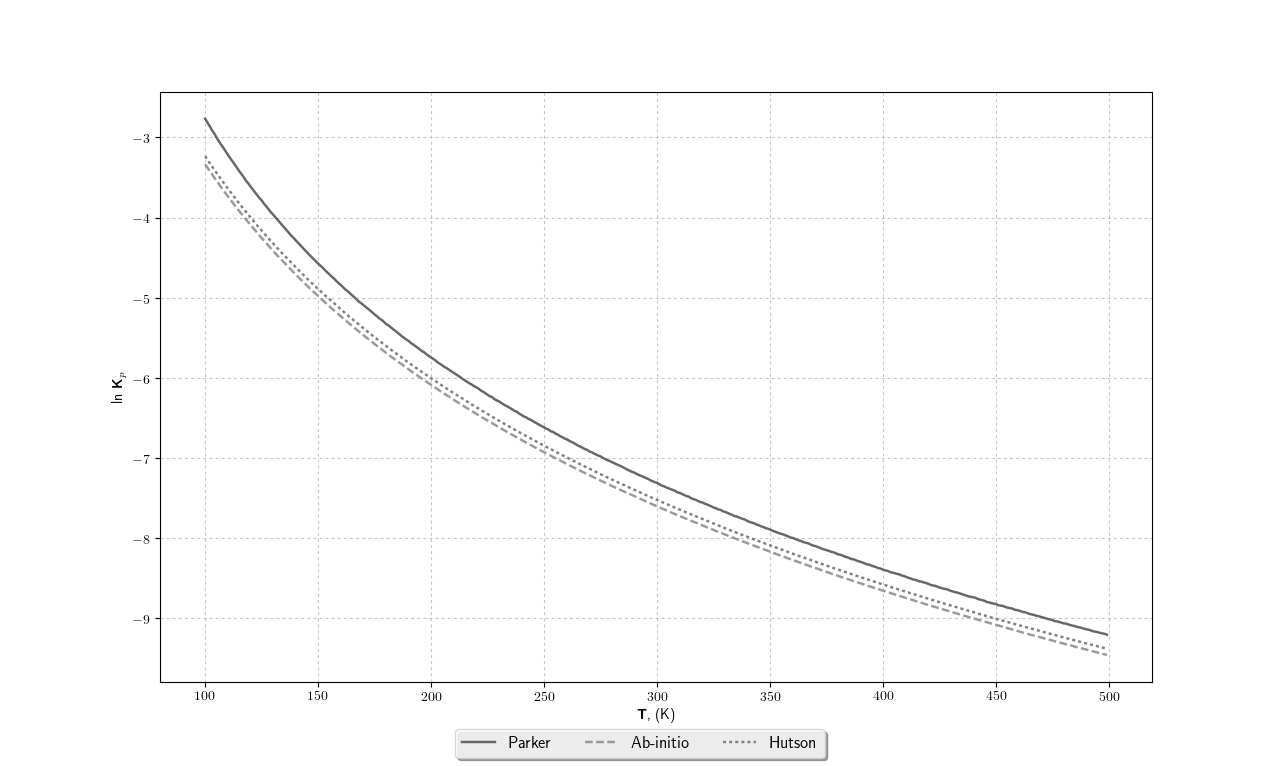
\includegraphics[width=\linewidth]{../pictures/all_eq_const.png}
\vspace*{-0.40cm}
\caption{\centering \scalebox{0.8}{Температурная зависимость логарифма константы равновесия}}
\end{figure}
\end{frame}

\begin{frame}{\normalsize Выводы}
\fontsize{8pt}{10}\selectfont
\begin{itemize}
 \item Описан метод получения точного классического колебательно-вращательного гамильтониана. Получен точный классический колебательно-вращательный гамильтониан системы $Ar-CO_2$.
 \item Выполнен расчет температурной зависимости второго вириального коэффициента с учетом первых квантовых поправок. Расчет проведен с использованием наиболее точной поверхности потенциальной энергии, полученной в [1]  методом \textit{ab initio}.  
 \item Основываясь на методе, развитом в [2], выражение для константы равновесия системы $Ar-CO_2$ было сведено к двумерному интегралу по области $U < 0$. 
 \item Была построена вычислительная схема, основанная на алгоритме адаптивного интегрирования по Монте-Карло [3, 4], позволяющая вычислять константу равновесия интегрированием по преобразованному фазовому пространству $\left\{ \mf{q}, \mf{p}, \mf{J} \right\}$, не используя упрощающих аналитических техник. 
  \item Расчет температурной зависимости константы равновесия выполнен двумя способами, и показано, что результаты этих расчетов идентичны.
\end{itemize}

\begin{flushleft}
	\textit{[1]}: Ю. Н. Калугина. Готовится к печати. 2017. \\
	\textit{[2]}: I. Buryak and A. Vigasin. Classical calculation of the equilibrium constants for true bound dimers using complete potential energy surface. \textit{J. Chem. Phys.}, \textbf{143}, 2015. \\
	\textit{[3]}: G. P. Lepage. \textit{J. Comput. Phys.}, \textbf{27}, 1978. \\
	\textit{[4]}: G. P. Lepage. Vegas. https://github.com/gplepage/vegas, 2013.
\end{flushleft}
\end{frame}

\begin{frame}{}
  \centering \Large
  \emph{Спасибо за внимание!}
\end{frame}

\end{document}
